\documentclass[10pt, a4paper]{aqademic}

\usepackage[spanish]{babel}
	\selectlanguage{spanish}

% Document packages

\usepackage[type=CC, modifier=by-nc-sa, version=4.0]{doclicense}
\usepackage{graphicx}
	\graphicspath{{img/}}

% Document settings

\author{Atanasio José Rubio Gil}
\title{Desarrollo de Software}

\AqSetChapter{Parte}

% Document composition

\begin{document}

\AqMaketitle[%
	author   = Atanasio José Rubio Gil,
	cover    = logo-ugr.png,
	org      = Grado en Ingeniería Informática,
	subtitle = Seminario de \texttt{git} y GitHub,
	url      = https://github.com/Groctel/ugr-informatica
]
% \tableofcontents

Llevo usando tanto \texttt{git} como GitHub desde algo antes de entrar en la carrera.
En este tiempo he alojado en la página varios proyectos en diversos lenguajes y he personalizado mi página principal para presentarme de forma elegante a la gente que me encuentre.
En este último año he creado y publicado varios proyectos de software libre disponibles en GitHub como:

\begin{itemize}
	\item\textbf{aqademia:}
		Una plantilla de {\LaTeX} (la que utilizo para estos trabajos).
	\item\textbf{dotfiles-manager:}
		Un gestor de ficheros de configuración escrito en shell.
	\item\textbf{vim-keytree:}
		Un plugin de Vim que emula la funcionalidad de \textit{which key} en Emacs.
\end{itemize}

\begin{figure}[ht!]
\begin{center}
	
\includegraphics[scale=0.25]{Seminario-git/perfil.png}
	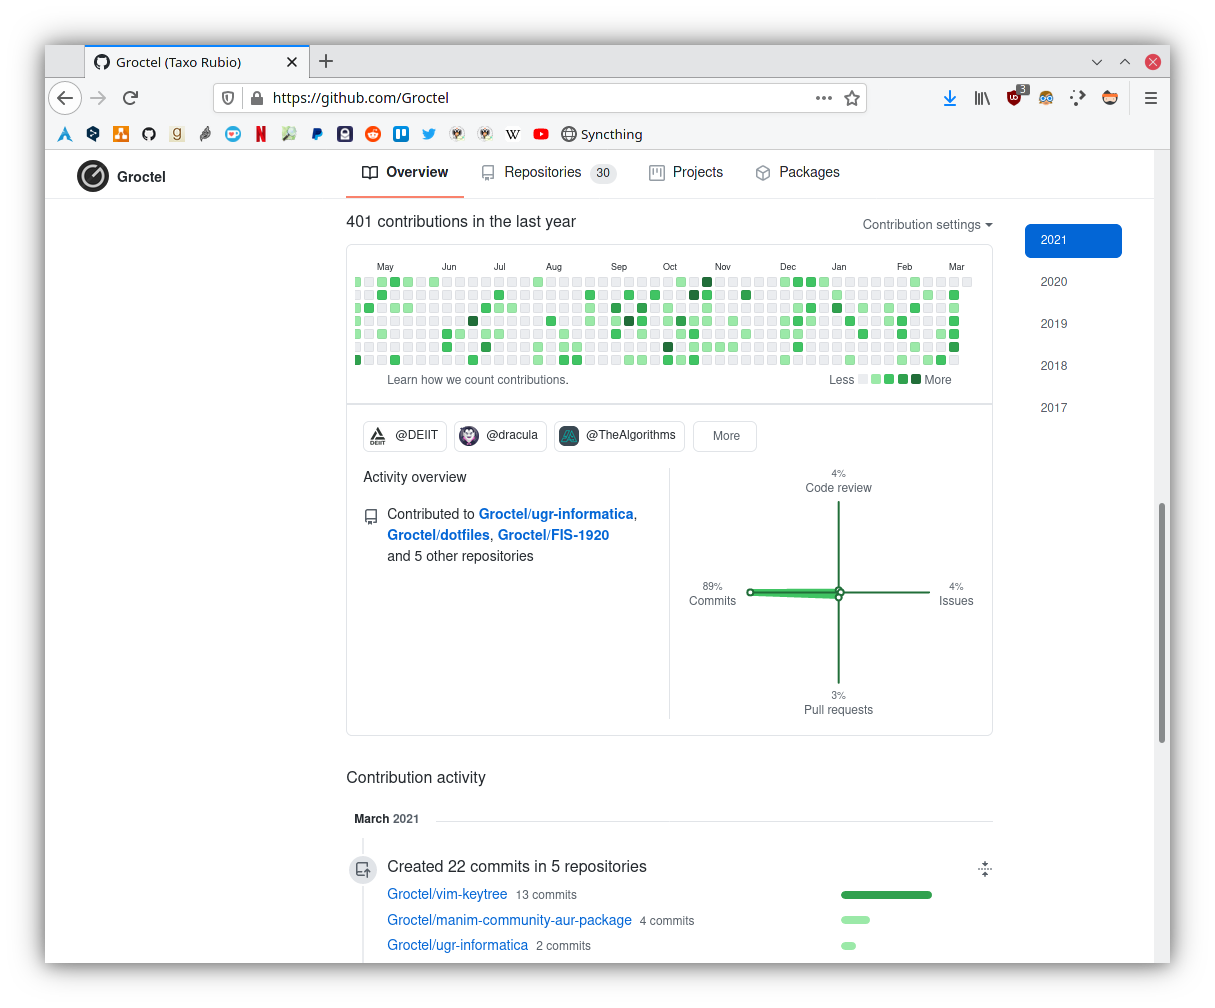
\includegraphics[scale=0.25]{Seminario-git/actividad.png}
\end{center}
\caption{Página personalizada de mi perfil de GitHub y mi historial de \textit{commits}.}
\end{figure}

Uno de los proyectos subidos a los que más apego le tengo es a Aqademia, ya que es una plantilla que uso de forma casi diaria.
El repositorio tiene bastante buena acogida aunque no lo he publicitado demasiado (principalmente entre mis conocidos en forma de boca a boca) y ha recibido alguna que otra propina.

\begin{figure}[ht!]
\begin{center}
	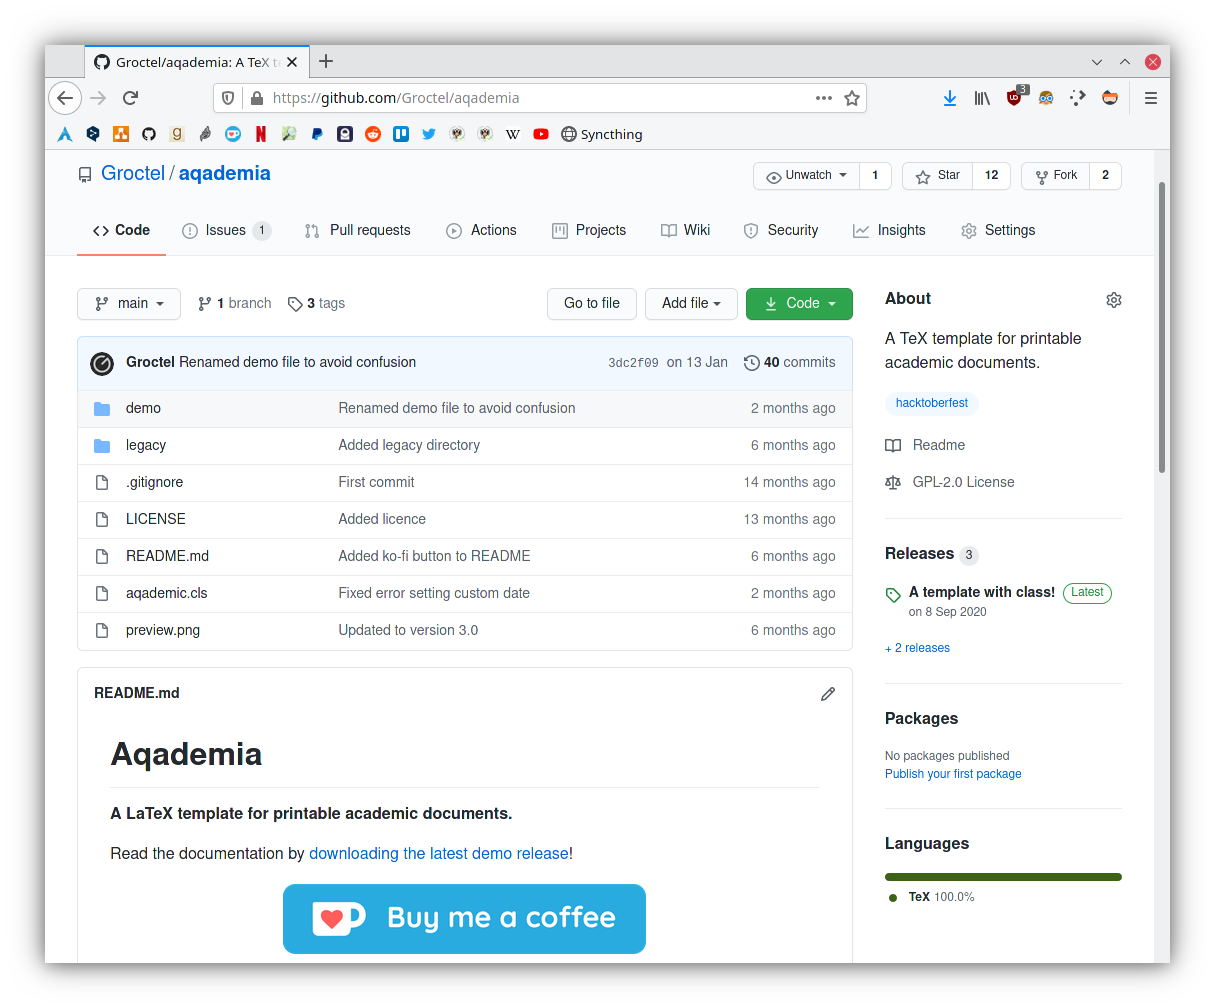
\includegraphics[scale=0.25]{Seminario-git/repositorio.png}
	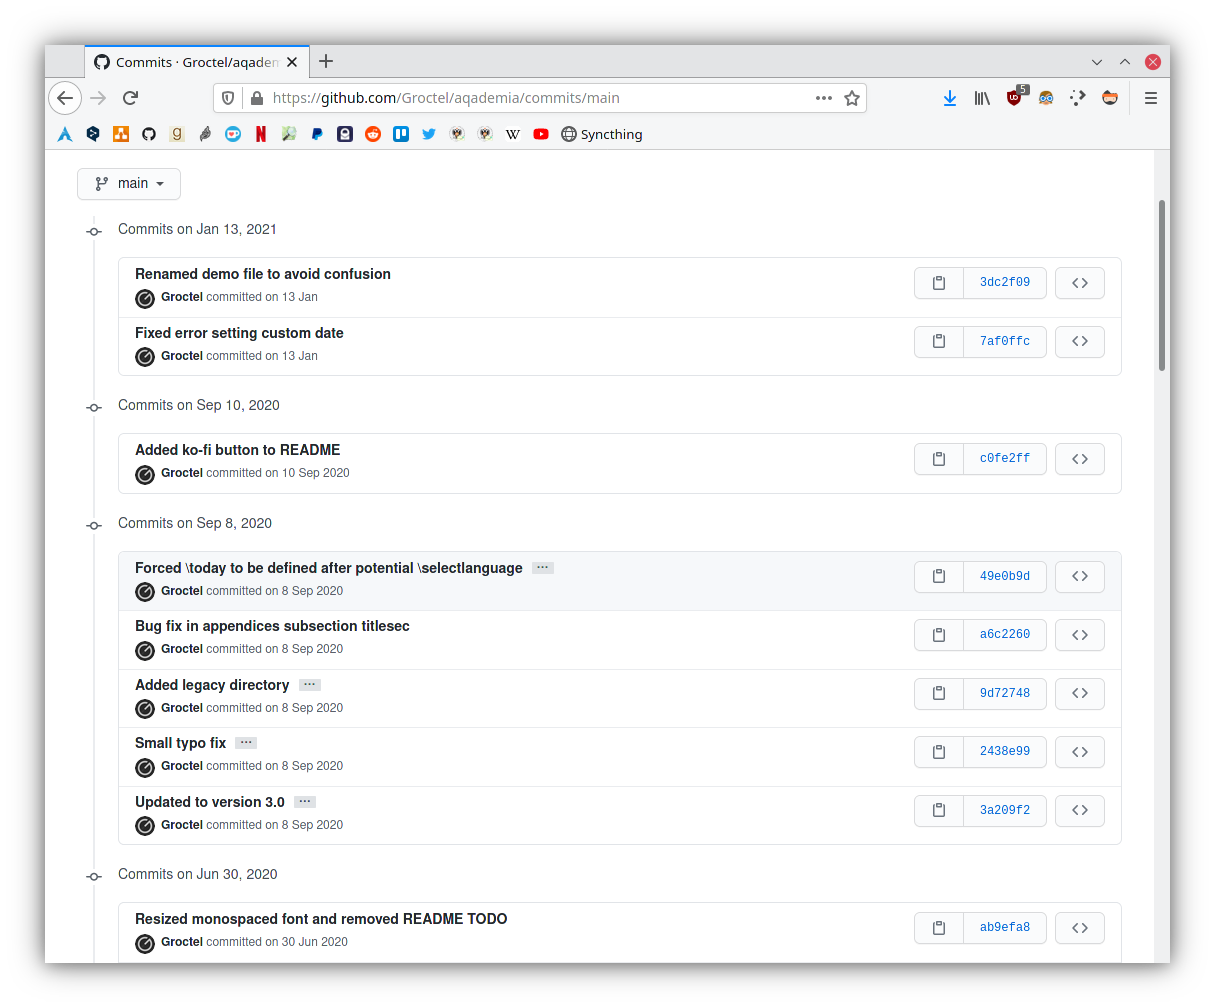
\includegraphics[scale=0.25]{Seminario-git/commits.png}
\end{center}
\caption{¡El repositorio de Aqademia tiene dos \textit{forks}!}
\end{figure}

\pagebreak

También tengo un repositorio específico de la carrera en el que almaceno todos los ficheros de código fuente del trabajo que voy realizando que cuenta con más de 100 commits en la rama \texttt{main}.
La estrategia que sigo para organizar las asignaturas es crear una rama distinta para cada una y fusionarla con la principal según las vaya acabando, de forma que todo lo que haya en \texttt{main} sea compilable.
Cabe destacar que los trabajos que realizo en otros repositorios los importo como submódulos, de forma que la forma de hacer \texttt{clone} y \texttt{pull} es particular a este caso y se encuentra documentada en el \texttt{README}.

\begin{figure}[ht!]
\begin{center}
	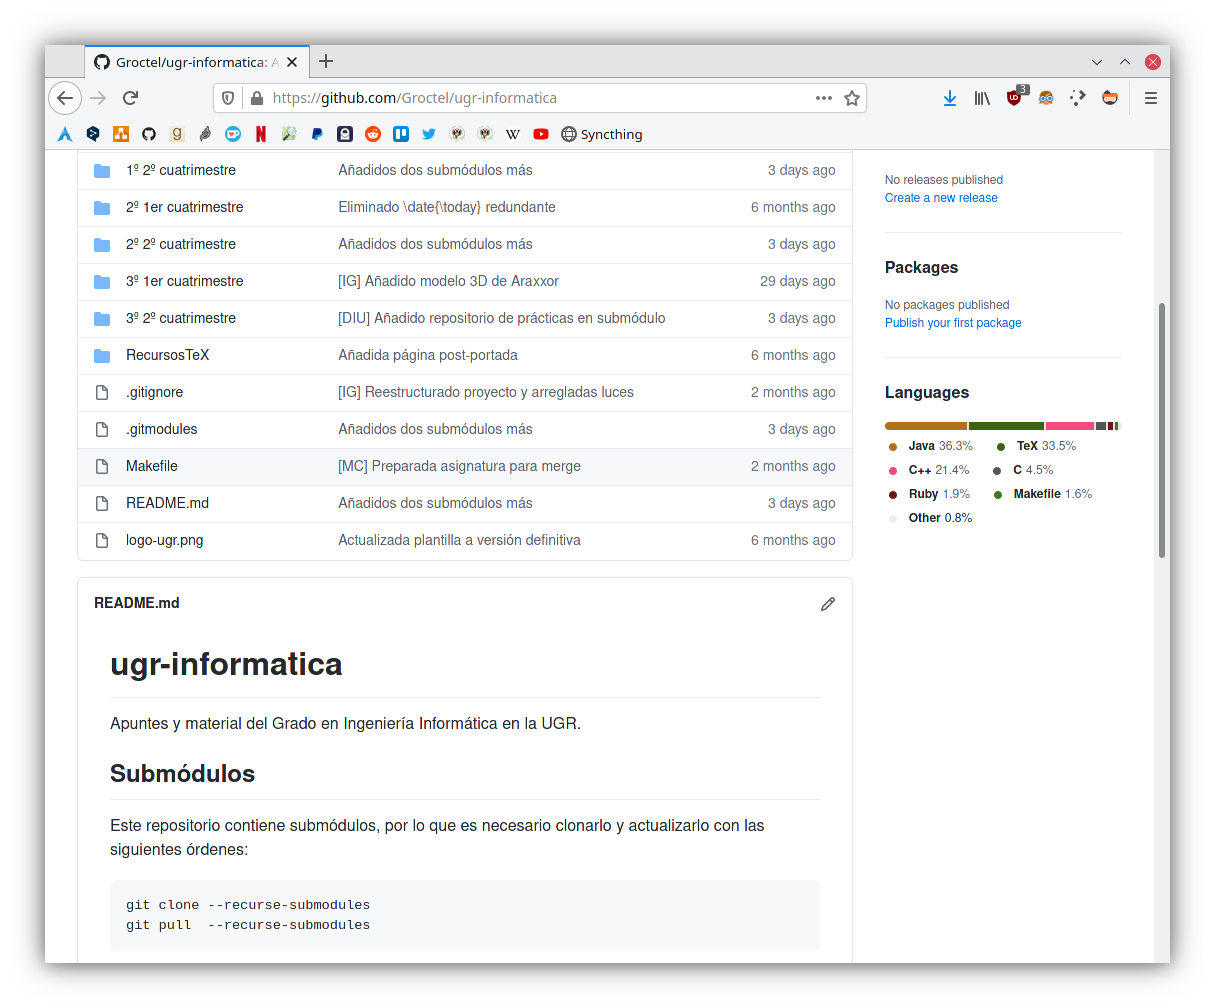
\includegraphics[scale=0.25]{Seminario-git/ugr-informatica.png}
	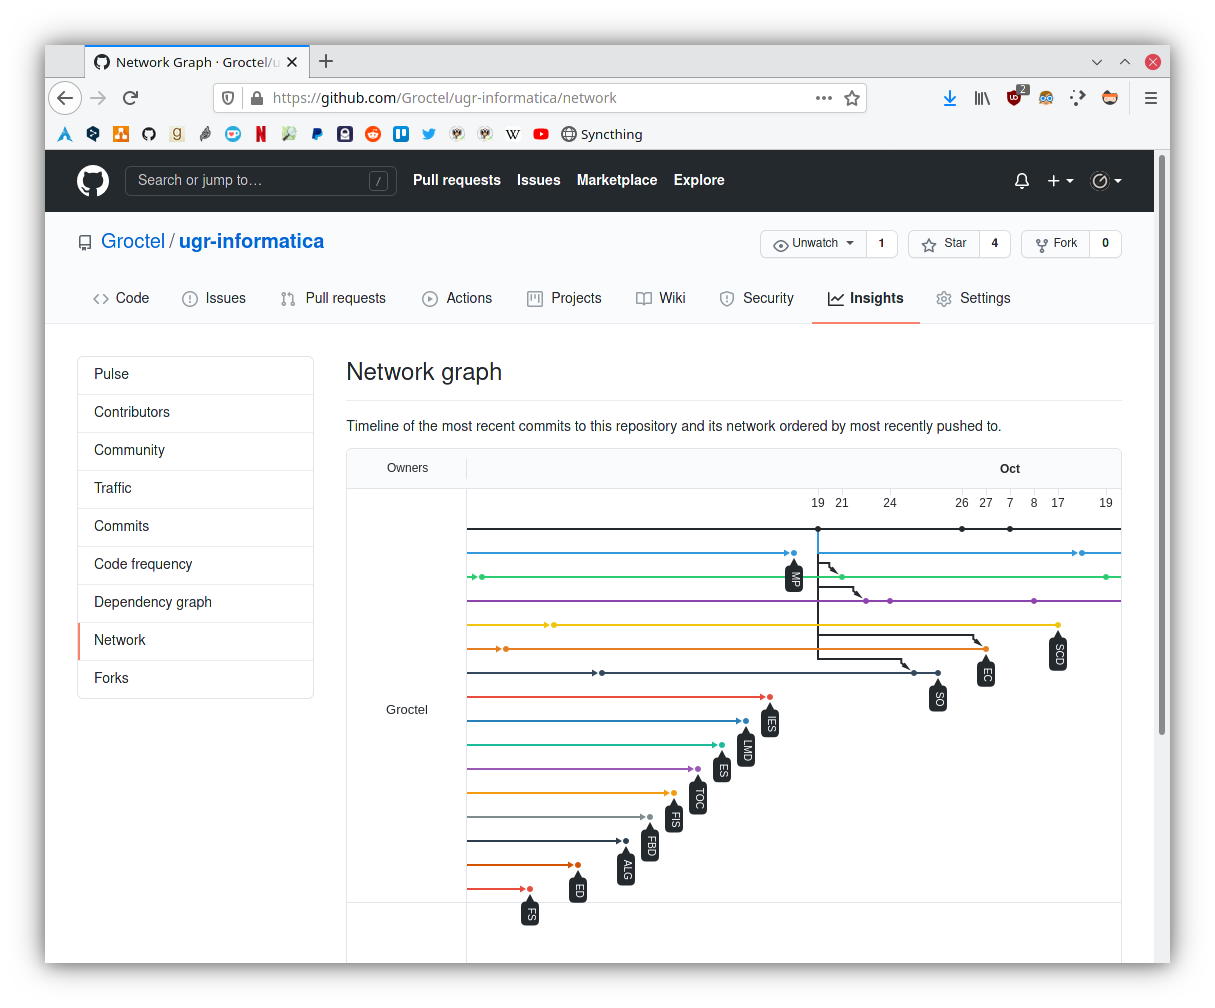
\includegraphics[scale=0.25]{Seminario-git/ramas.png}
\end{center}
\caption{Mi repositorio \texttt{ugr-informática} organiza las asignaturas por ramas.}
\end{figure}

Dado que en GitHub se almacenan proyectos de software, he trabajado con las versiones o \textit{releases} de mis proyectos.

\begin{figure}[ht!]
\begin{center}
	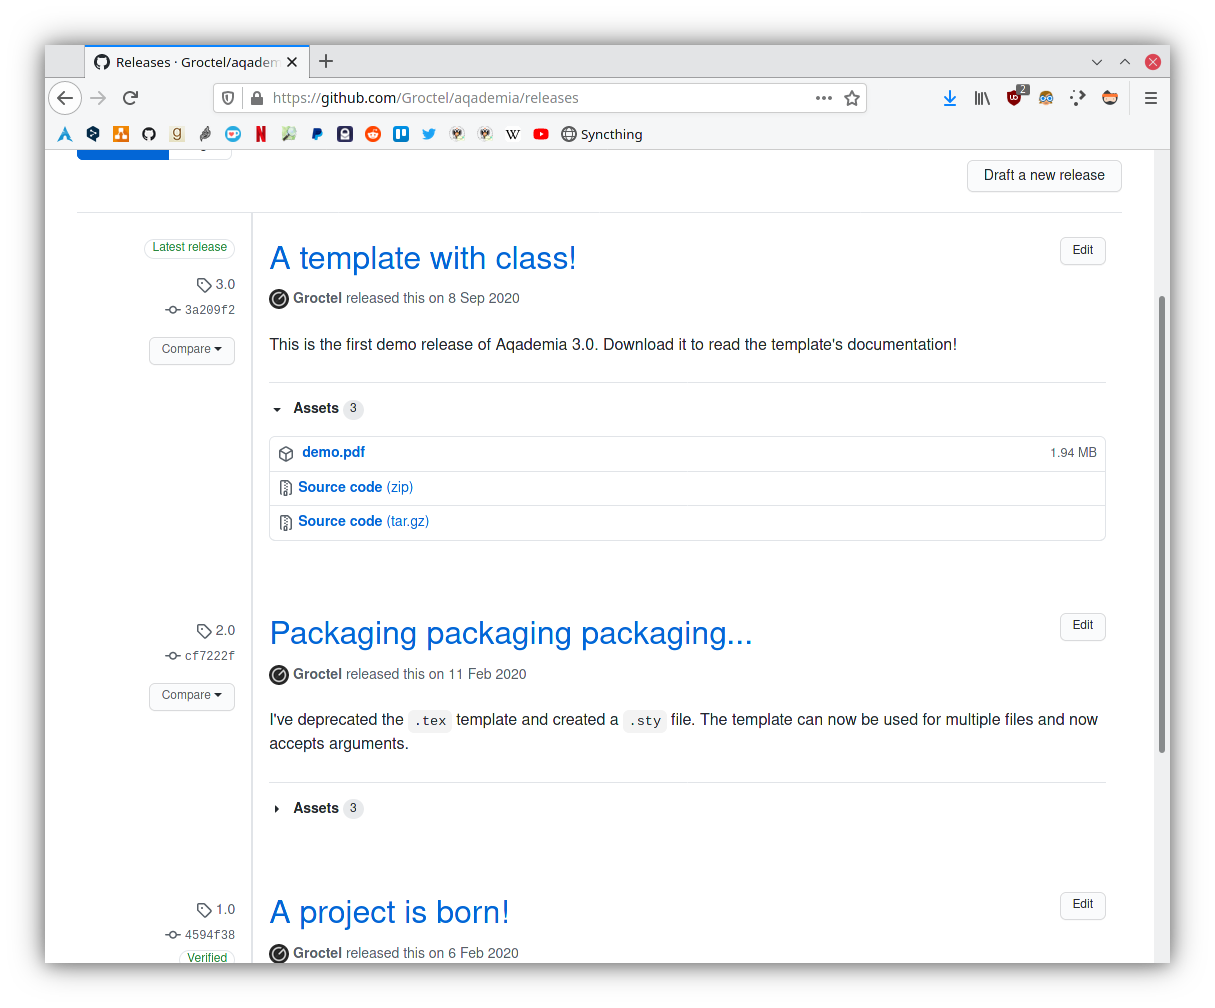
\includegraphics[scale=0.25]{Seminario-git/releases.png}
\end{center}
\caption{Aqademia cuenta con tres versiones que, por desgracia, no pude hacer retrocompatibles.}
\end{figure}

\pagebreak

Por último, aunque no menos importante, también he trabajado con \textit{issues} y \textit{pull requests}.

\begin{figure}[ht!]
\begin{center}
	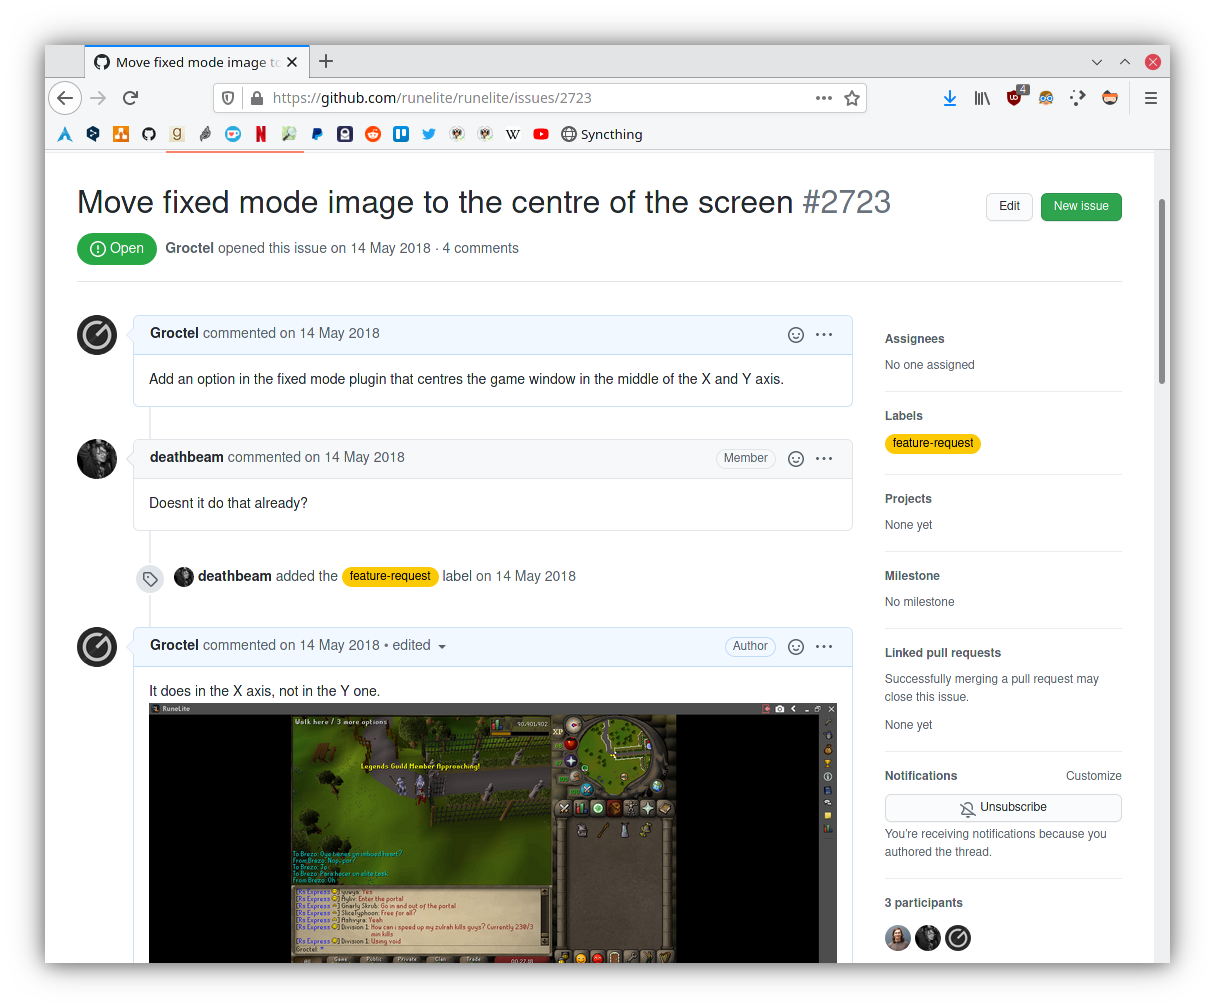
\includegraphics[scale=0.25]{Seminario-git/issue.png}
	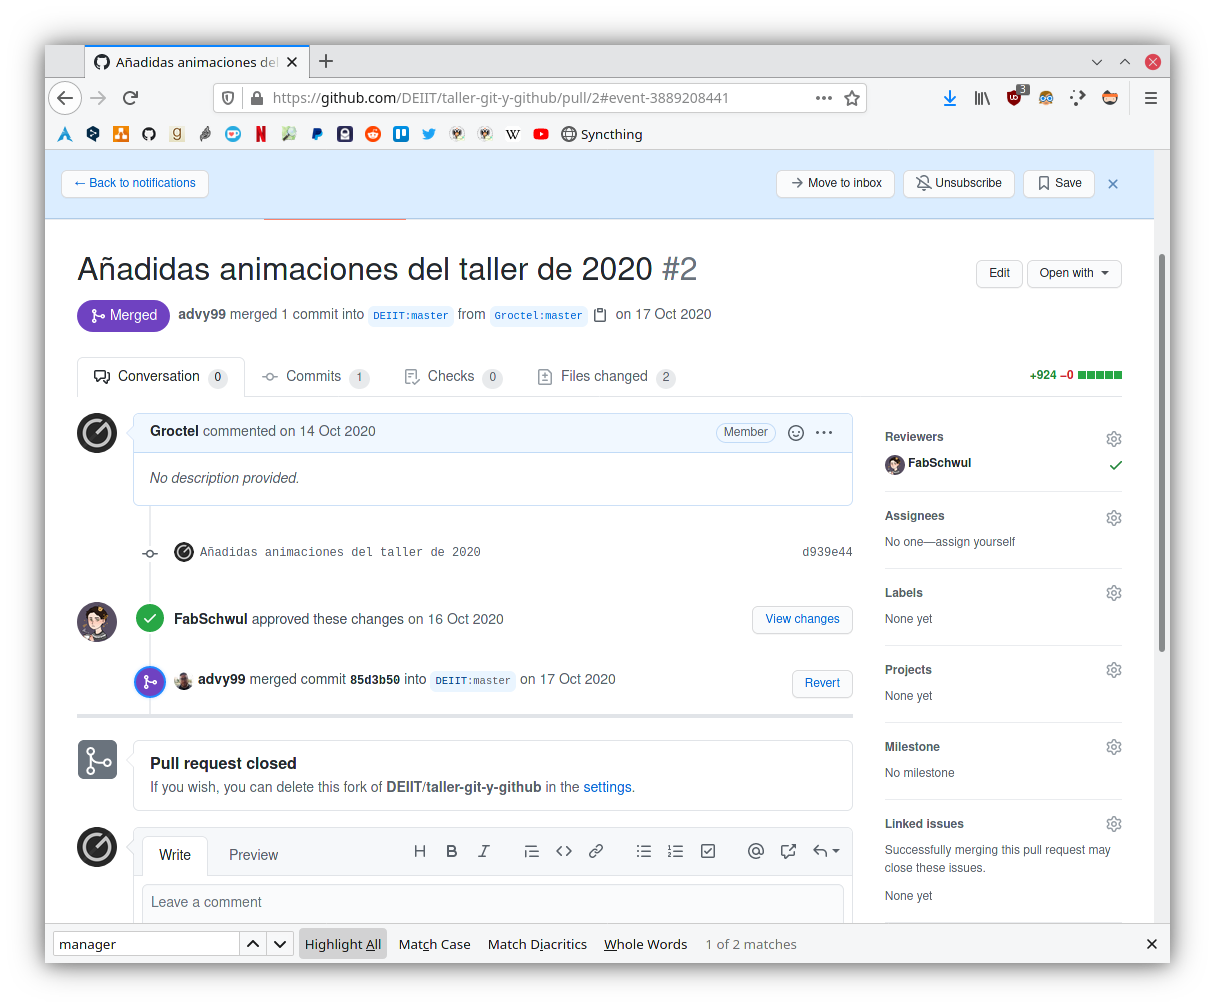
\includegraphics[scale=0.25]{Seminario-git/pr.png}
\end{center}
\caption{Las herramientas de colaboración de GitHub son muy cómodas de utilizar.}
\end{figure}

Este documento está escrito en {\LaTeX} y su código se encuentra alojado en la rama \texttt{DS} de mi repositorio \texttt{ugr-informatica}, enlazado en la portada.

\end{document}
